\documentclass[spanish]{article}
\usepackage[spanish]{babel}
\usepackage{amsmath}
\usepackage{amssymb}
\usepackage[utf8]{inputenc}
\usepackage{vmargin}
\usepackage{graphicx}
\usepackage{wrapfig}
\usepackage[export]{adjustbox}


\begin{document}
	\setpapersize{USletter}
	\setmarginsrb{30mm}{30mm}{30mm}{30mm}{0pt}{0mm}{0pt}{0mm}
	
	\begin{center}
	{\Large Análisis de Algoritmos, Sem: 2018-1, 3CV2 Práctica 6, 19 de Octubre del 2017}\\
{\huge {\bf Práctica 6: Problema del Maximo Subarreglo}} \\
{\huge {\bf Martínez Berumen Luis Daniel}} \\

\includegraphics[width=1\textwidth, right]{./imagenes/logos.png}
	\end{center}
	
	\bigskip
	
	\bigskip
	
	\bigskip
	
	{\LARGE {\bf Abstract}}\\
	
	En esta practica analizaremos la complejidad del algoritmo de maximo subarreglo, de igual manera la complejidad del maximo subarreglo cruzado, estos seran tratados tanto de manera grafica como de manera analitica, esperamos que los resultados sean de un algoritmo con complejidad lineal, para el caso del maximo subarreglo cruzado, en el caso del algortimo de maximo subarreglo una complejidad de $\theta(nlogn)$, ademas de considerar el caso cuando el arreglo esta lleno con numeros enteros negativos, en el cual sabemos se presenta un caso interesante para su analisis.

	\bigskip

	{\Large {\bf Palabras Clave}}\\
	\begin{itemize}
		\item Algoritmo
		\item Funcion
		\item Recursividad
		\item Orden
		\item Arreglo
	\end{itemize}

	\section{Introducci\'on}
Divide y Vencerás es una frase quye hemos escuchado todos, al menos, una vez en nuestra vida, para nosotros 
	es técnica de diseño de algoritmos, siendo de gran utilidad para nuestra carrera, ya que, 
	los problemas a los que nos enfrentamos día con día son mas faciles de resolver si aplciamos una tecnica de este tipo.
	De hecho, suele ser considerada una filosofía general para resolver problemas, no solo del termino informatico, sino que también           se utiliza en muchos otros ámbitos

\newpage
	\section{Conceptos B\'asicos}
	Para la correcta comprension de este trabajo, es necesario definir algunos terminos tales como $\theta$, O y $\Omega$.\\
	 $\theta$(n):\\
		Sea g(n) una función. Se define  $\theta$ (g(n)) como:\\
		
		 	$\theta$(g(n)) = $\{ f(n) \quad | \quad \exists c1,c2>0 \quad \& \quad n_{0}>0 \quad \mid \quad \forall n>=n_{0} \quad 0<= c1g(n) <= f(n) <= c2g(n) \}$
	\bigskip		 	
		 	
	O(n):\\
		Sea  g(n)  una función, O(n) (el pero de los casos) se define como:\\
		
			\hspace{1cm}O(n)=$\{f(n) \quad | \quad \exists c >0 \quad \& \quad n_{0}>0 \quad | \quad f(n) <= Cg(n) \quad \forall  n>= n_{0} \}$
	\bigskip
	
	$\Omega$(n):\\
	Sea  g(n)  una función. Se define $\Omega$ (g(n)) (el mejor de los casos) como:\\

		\hspace{1cm}$\Omega$(g(n)) =$\{f(n) \quad | \quad \exists c >0 \quad \& \quad n_{0}>0 \quad \mid \quad  0<= cg(n)<= f(n) \quad \forall n>= n_{0} \}$
	\bigskip

	El problema del subarreglo máximo consiste en encontrar un subarreglo de una determinada longitud m cuya suma sea máxima dentro de un arreglo de longitud n, con m mayor a n.\\
	\begin{center}
		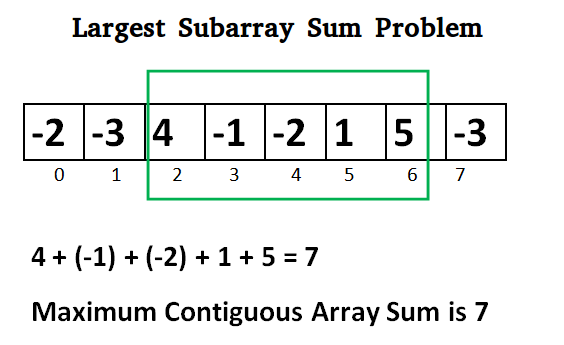
\includegraphics[width=0.55\textwidth]{./imagenes/fig1.png}\\
		Figura 1 Maximo SubArreglo .\\
	\end{center}
	En la figura 1, podemos apreciar que tenemos un arreglo de 8 elementos, podemos ver que consta de numeros tanto negativos como positivos, pero siempre enteros.\\
Como podemos ver, la suma de los elementos en las posicions 2 a 6, nos da un resultado de 7, a este arreglo se le llama maximo subarreglo, ya que es la maxima suma obtenible con elementos secuenciales dentro del arreglo.
	
	\newpage	

	\section{Experimentaci\'on y Resultados}
	
	\subsection{Implemente el algortimo del maximo subarreglo.}
	
	{\large{ {\bf i) Mediante gráficas, muestre que el algoritmo de  ${\bf maximo subarreglo cruzado}$ tiene complejidad lineal.}}}\\

	\bigskip

	\begin{center}
		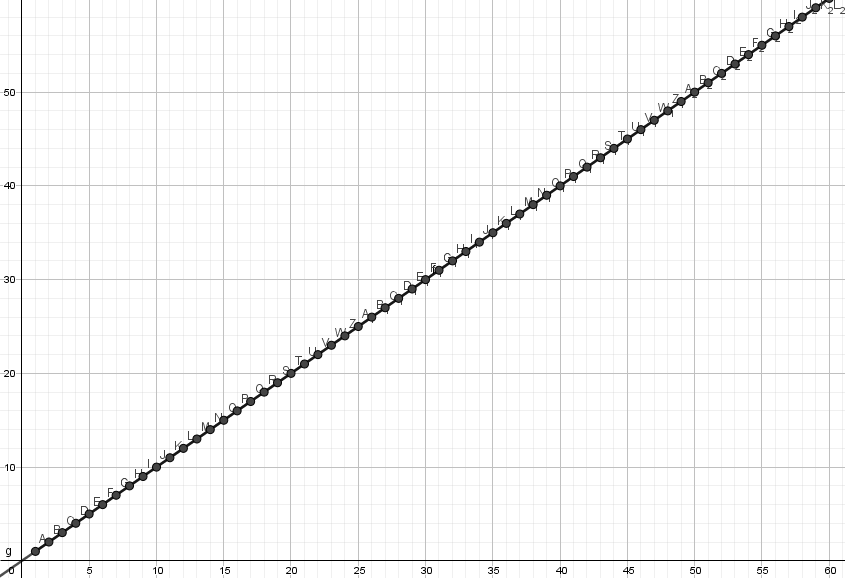
\includegraphics[width=0.60\textwidth]{./imagenes/msc.png}\\
		Figura 2. Gráfica del algoritmo del máximo subarreglo cruzado.\\
	\end{center}


	\bigskip

La curva de color negro es la función f(n) que propongo apartir de los resultados obtenidos de la ejecución,y  la recta de color verde es g(n). Como se puede observar en la figura 2, tanto la función propuesta como la función obtenido por medio del algoritmo se enciman, es decir, se puede concluir de manera gráfica que el algoritmo del máximo subarreglo cruzado tiene de cota superior lineal. Dicha función es de tipo T(n)=${\theta(n)}$.\

	\bigskip
\newpage
	{\large{\bf ii)  Demuestre analíticamente que el algoritmo  ${\bf maximo subarreglo cruzado}$ tiene complejidad lineal.}}\\
	
	\bigskip
	
	MSC(A, bajo, medio, alto)  \hspace{4cm} Costo\\
    	1.-sumaIzq $ \leftarrow \infty $ \hspace{6cm} 1\\
    	2.-suma$ \leftarrow 0 $ \hspace{7cm} 1\\
    	3.-for i=medio to i=bajo \hspace{4cm} medio-bajo+2\\
    	4.-\hspace{0.5 cm} suma $ \leftarrow $ suma +A[i] \hspace{4.5cm} 1\\
    	5.-\hspace{0.5cm} if suma $ \> $ sumaIzq \hspace{5cm} 1 \\
    	6.-\hspace{1cm} sumaIzq $ \leftarrow $ suma \hspace{4.5cm} 1 \\
    	7.-\hspace{1cm} maxIzq $ \leftarrow $ i \hspace{5.5cm} 1 \\
        8.-sumaDer $ \leftarrow \infty $ \hspace{6cm} 1\\
    	9.-suma$ \leftarrow 0 $ \hspace{7cm} 1\\
        10.-for i=medio+1 to i=alto \hspace{4cm} alto-(medio+1)+2\\
    	11.-\hspace{0.5 cm} suma $ \leftarrow $ suma +A[i] \hspace{4.2cm} 1\\
    	12.-\hspace{0.5cm} if suma $ \> $ sumaDer \hspace{4.5cm} 1 \\
    	13.-\hspace{1cm} sumaDer $ \leftarrow $ suma \hspace{4cm} 1 \\
    	14.-\hspace{1cm} maxDer $ \leftarrow $ i \hspace{5cm} 1 \\
    	
    	\noindent medio-bajo+2+alto-medio-1+2 \\
    	= alto-bajo+3 \\
    	= alto-bajo+1+2 \\
    	= n+2 \\
    	= $ \theta (n) $

	\bigskip
\newpage

	{\large{\bf iii) Mediante gráficas, muestre que el algoritmo  ${\bf maximo subarreglo }$ tiene complejidad ${\bf \theta(nlogn)}$.}}\\
	
	\bigskip
	
	\begin{center}
		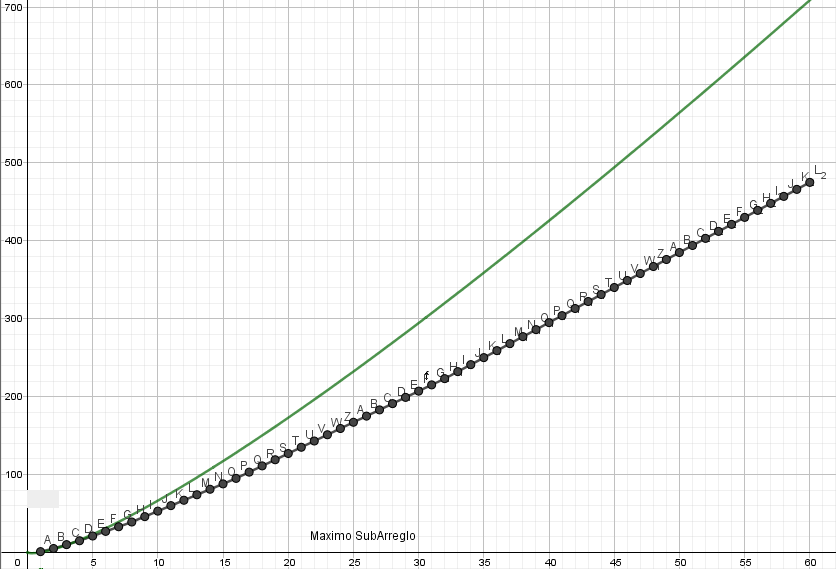
\includegraphics[width=0.55\textwidth]{./imagenes/ms.png}\\
		Figura 3. Gráfica del algoritmo del máximo subarreglo.\\
	\end{center}

	\bigskip

La curva de color negro es la función f(n) que propongo apartir de los resultados obtenidos de la ejecución,y tiene un comportamiento muy similar al de T(n)=${\theta(nlogn)}$, mientras la recta de color verde será nuestra g(n) será muy similar a f(n) con la única diferencia que será multiplicado por alguna constante C. Observando la figura 3 se puede notar que  nuestra cota superior propuesta para el algoritmo del máximo subarreglo es la correcta. Por lo tanto, es correcto suponer que el algoritmo tiene complejidad de la forma T(n)=${\theta(nlogn)}$.\\

	\bigskip
\newpage

	{\large{\bf iV) Demuestre  analíticamente que el algoritmo  ${\bf maximo subarreglo }$tiene complejidad ${\bf \theta(nlogn)}$.}}
	
	\bigskip
	
	1.-if bajo=alto \hspace{6cm} $ \theta(1) $ \\
        2.-\hspace{0.5cm} return(bajo, alto A[bajo]) \hspace{3cm} $ \theta(1) $ \\
        3.-else \\
        4.-medio $ \leftarrow $ (bajo+alto)/2 \hspace{5cm} 1 \\
        5.-MS(A, bajo, medio) \hspace{5.5cm} $ T(\frac{n}{2}) $ \\
        6.-MS(A, medio+1, alto) \hspace{5cm} $ T(\frac{n}{2}) $ \\
        7.-MSC(A, bajo, medio, alto) \hspace{4cm} $ \theta (n) $ \\
        8.-if(sumaIzq $ \< $ sumDer $ \& $ sumaIzq $ \> $ sumaCruz)  \hspace{1cm} $ \theta (1) $\\
        9.-return(mmIzq, maxIzq, sumaIzq)  \hspace{3cm} $ \theta (1) $\\

	\bigskip
\newpage
	{\large{\bf V) Implemente un algoritmo que resuelva el problema del máximo subarreglo utilizando fuerza bruta. Calculé su orden de complejidad analítica y experimentalmente.}}\\
	
	\bigskip
	
	\begin{center}
		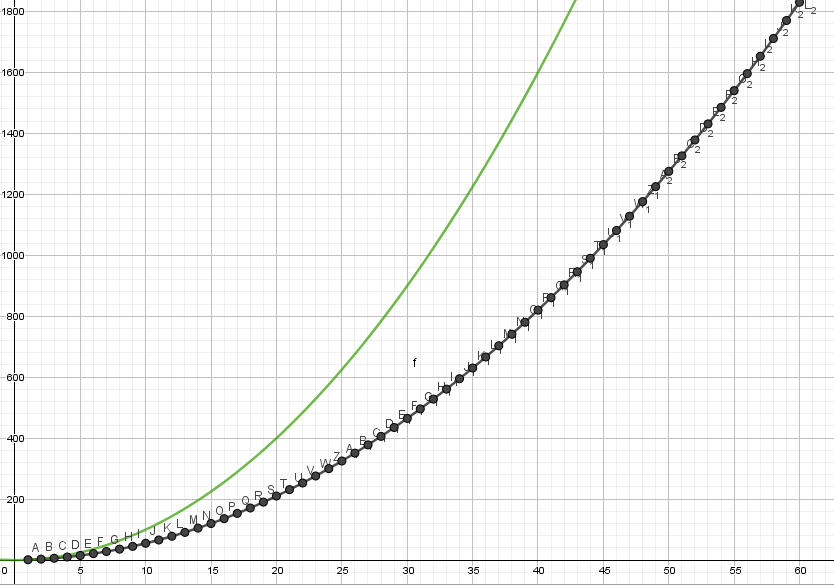
\includegraphics[width=0.55\textwidth]{./imagenes/fb.png}\\
		Figura 4. Gráfica del algoritmo implementado por l fuerza bruta.\\
	\end{center}

	\bigskip

La curva de color negro es la funcion f(n) que propongo apartir de los resultados obtenidos por medio de la experimentación y g(n) será la recta de color verde. El comportamiento que vamos a proponer será de T(n)=${\theta(n^{2})}$, tanto f(n) como g(n) se puede verificar que dicha complejidad sirve como cota superior de manera correcta. Por lo tanto, dicho algoritmo es de la forma T(n)=${\theta(n^{2})}$

	\bigskip

	\newpage

	\bigskip

	\section{Conclusi\'on}

	\bigskip

	Para estra practica regrese a utilizar C, ya que, al utilizar arreglos, la manera de C de manipularlos me sigue pareciendo mas sencilla que Python.\\Me doy cuenta que en esta practica no es solamente necesario suponer que algun algoritmo tiene cierta complejidad, debemos de tener algun analisis, ya que es importante respaldar toda nuestra hipotesis con informacion verdadera.\\Este algoritmo, cuando lo analise a "Ojo de buen cubero" no creia que fuera asi de complicada su implementacion, tuve que regresar a un lenguaje en el que me siento mas comodo como lo es C, esta vez Python no me ayudo tanto. Me gusto el trabajo de implementar este algoritmo, siento que fue la mejor manera de cerrar el tema de "Divide y venceras".

	\bigskip


	\newpage

	\bigskip

	\section{Bibliografía}
	\begin{itemize}
		\item Brassard, G. (1997). Fundamentos de Algoritmia. España: Ed. Prentice Hall. ISBN 		848966000X
		\item Harel, D. (2004). Algorithmics: The spirit of Computing (3rd. Ed). Estados Unidos de América: Addison
Wesley. ISBN-13: 978-0321117847
	\end{itemize}


\end{document}